\chapter{Design Del Sistema}
\section{Descrizione dell'architettura}
BugBoard26 adotta un'architettura software a tre livelli, separando Frontend, Backend e Database, pensata per distinguere la logica di presentazione da quella dell'accesso dei dati.


\begin{table}[h]
\begin{tabular}{|c|l|}
\hline
\rowcolor[HTML]{FFFFFF} 
\textbf{Livello}                                & \multicolumn{1}{c|}{\cellcolor[HTML]{FFFFFF}\textbf{Descrizione}}                                                                                                                                                 \\ \hline
\rowcolor[HTML]{C4C4C4} 
{\color[HTML]{000000} Presentazione (Frontend)} & {\color[HTML]{000000} \begin{tabular}[c]{@{}l@{}}Applicazione lato client,responsabile dell'interfaccia \\ e dell'interazione con l'utente\end{tabular}}                                                          \\ \hline
\rowcolor[HTML]{FFFFFF} 
{\color[HTML]{000000} Business Logic (Backend)} & {\color[HTML]{000000} \begin{tabular}[c]{@{}l@{}}Applicazione monolitica RESTful incaricata dell'elaborazione\\  delle richieste, della sicurezza, dell'autorizzazione e delle \\ regole di dominio\end{tabular}} \\ \hline
\rowcolor[HTML]{C4C4C4} 
Persistenza (Database)                           & \begin{tabular}[c]{@{}l@{}}Sistema relazionale utilizzato per la memorizzazione definitiva\\ e strutturata dello stato delle entità\end{tabular}                                                                  \\ \hline
\end{tabular}
\end{table}

\newpage
\subsection{Deployment diagram}
\begin{figure}[h!]
    \centering
    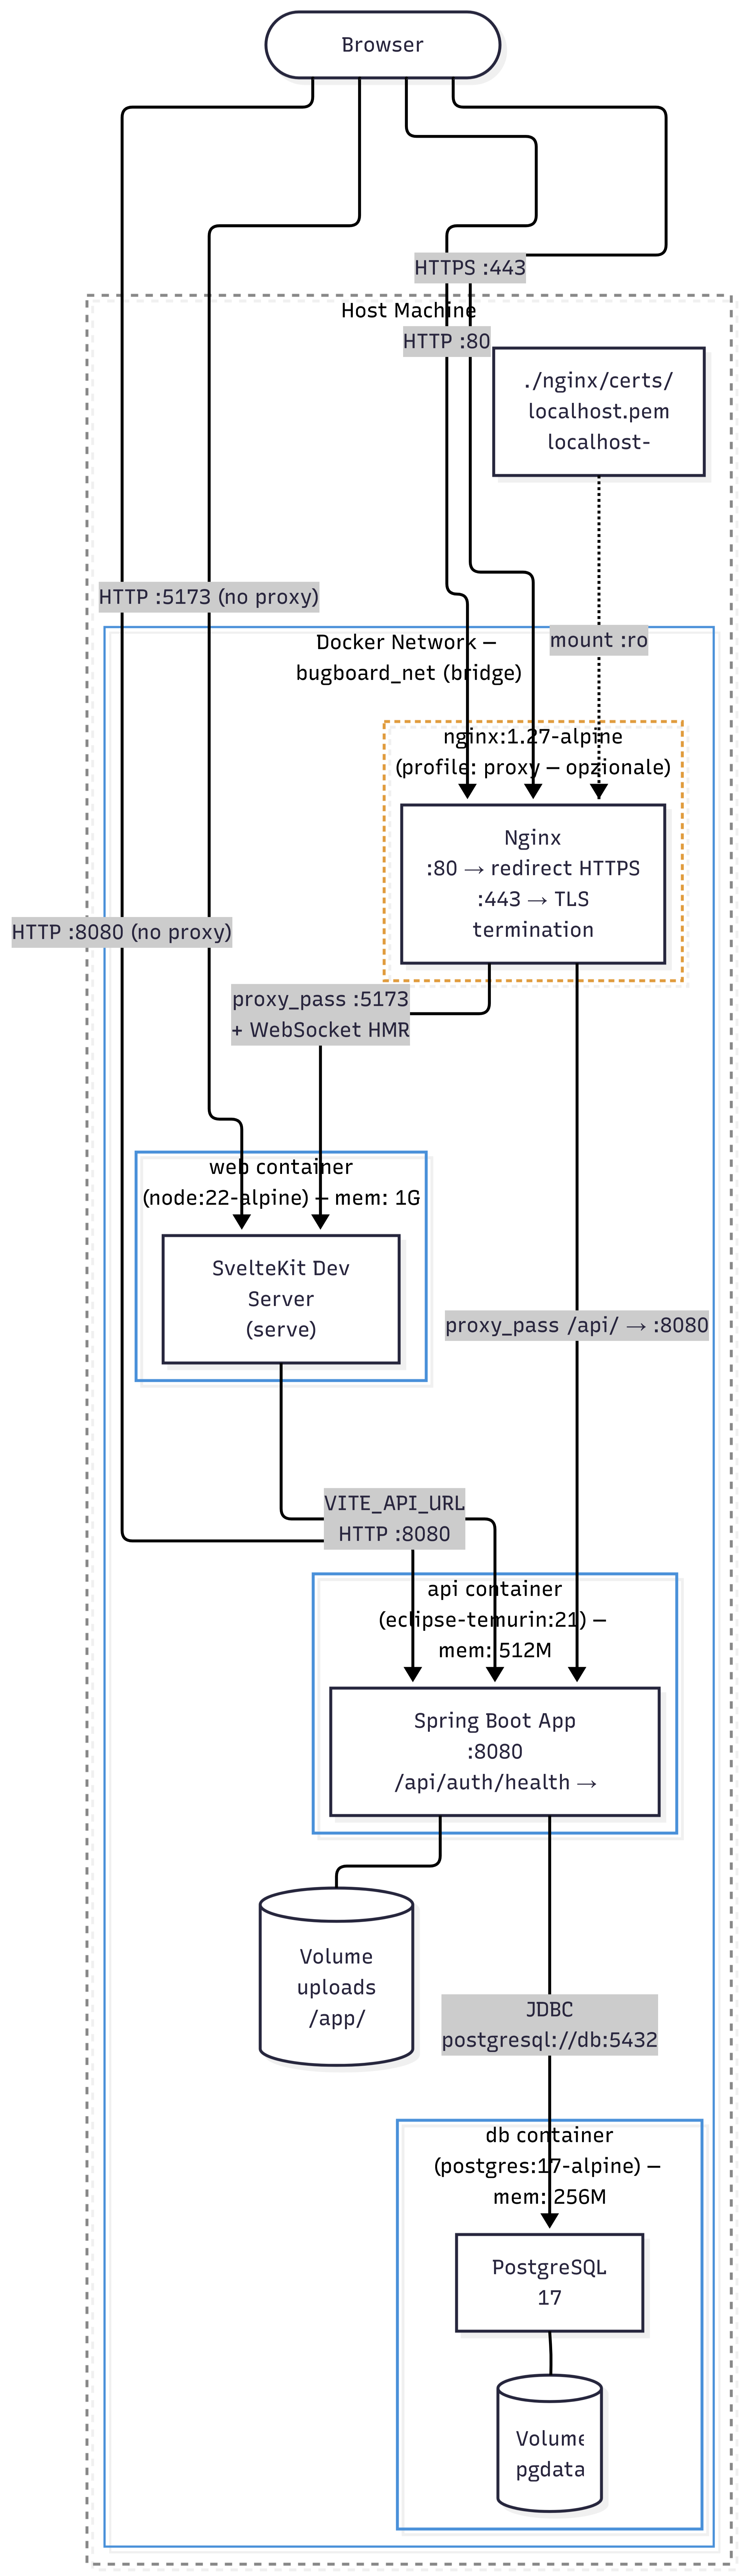
\includegraphics[width=0.42\linewidth]{AssetsDocumentazione/deployment.png}
    \caption{Deployment Diagram}
\end{figure}
\newpage

\section{Criteri di design adottati}

\begin{itemize}[itemsep=2pt]
    \item \textbf{Architettura a strati (Layered Architecture):} Le classi Spring boot sono suddivise gerarchicamente per evitare accoppiamenti forti: \\
    I \textit{Controller} gestiscono le risposte HTTP, i \textit{Service} incapsulano la logica applicativa, mentre i \textit{Repository} effettuano manipolazioni di basso livello sul database
    \item \textbf{Separation of Concerns (SoC):} L'infrastruttura client-server separa l'Interfaccia Utente dalle logiche di sistema, permettendo l'aggiornamento dei due moduli in modo indipendente
    \item \textbf{Autuenticazione Stateless:} Il tracciamento dell'identità viene effettuato usando JSON Web Token (JWT), token crittografati generati dal client durante il login  in comunicazione protetta
\end{itemize}

\section{Scelte tecnonlogiche}
\subsection{Frontend}
\begin{itemize}[itemsep=2pt]
    \item \textbf{Svelte 5 e SvelteKit:} Framework usati per generare codice JavaScript efficiente e ottimizzato in fase di compilazione 
    \item \textbf{Vite:} Tool scelto per rendere gli startup dell'ambiente di sviluppo quasi istantanei
    \item \textbf{Tailwind CSS:} Framework introdotto per una prototipazione scalabile, con aggiunta di plugin ufficiali per il reset form e tipografia avanzata
    \item \textbf{TypeScript:} usato nel client per garantire tipizzazione statica, al fine di prevenire bug in runtime
\end{itemize}

\subsection{Backend}
\begin{itemize}[itemsep=2pt]
    \item \textbf{Java 23:} Versione Java utilizzata, moderna, permette l'uso di Record, utilizzati per la mappatura dei Data Transfer Object (DTO)
    \item \textbf{Sprint Boot 3.4.2:} Framework utilizzato per applicazioni Java, permette di autoconfigurare le dipendenze e inizializzare servlet embedded
    \item \textbf{Spring Data JBA:} Basato su Hibernate, usato per definire le entità e automatizzare le query dinamiche
    \item \textbf{Spring Security e JJWT:} Moduli responsabili di autenticazione e autorizzazione, generazione e codifica di JSON Web Tokens
    \item \textbf{H2 Database:} Database relazionare in memoria, utilizzato per test rapidi e isolati
    \item \textbf{OpenCSV e iText Core 9.1.0:} Librerie di supporto per i documenti; consentono l'esportazione di statistiche in vari formati
\end{itemize}

\newpage

\subsection{Deployment e Sviluppo}
\begin{itemize}[itemsep=2pt]
    \item \textbf{Docker / Docker Compose:} Gestione di frontend, backend, database e isolamento dei servizi
    \item \textbf{Maven:} Gestione di dipendenze e build automaton per Java
\end{itemize}
\newpage

\section{Comunicazione fra livelli}
La comunicazione fra i vari livelli è basata sul protocollo HTTP/1.1, con scambio di payload in formato JSON decodificati automaticamente dal framework
\begin{itemize}[itemsep=2pt]
    \item \textbf{L'autenticazione} è passata in ogni richiesta HTTP dal client tramite l'header \textit{Authorization: Bearer <token\_jwt>}
    \item I\textbf{ flussi di esportazione} file restituiscono flussi binari o testo delimitato con i corretti header \textit{Content-Disposition}
    \item Le \textbf{transazioni} che prevedono operazioni in scrittura (creazione e modifica di \textit{Bug} o \textit{Utenti}) sfruttano richieste mappate su precisi DTO di convalida
\end{itemize}

\subsection{Sicurezza e Controllo degli Accessi}
\begin{itemize}[itemsep=2pt]
    \item \textbf{Storage sicuro di credenziali:} Le password inserite dagli Users non sono mai salvate in plaintext, bensì vengono offuscate con un \textit{encoder crittografico} (BCrypt). Per le successive comparazioni in fase di login, si usano delle stringe \textit{Hash}
    \item \textbf{Role-Based Access Control (RBAC):} Sistema basato su privilegi \textit{GlobalRole}, per cui tentativi di esecuzione di comandi non permessi vengono intercettati dal modulo \textit{PermissionService} e bloccati immediatamente, generando una \textit{AccessDeniedException} per il client
\end{itemize}